\section{Evaluation}\label{sec:evaluation}

The evaluation of our preemption point placement algorithm will embody
two methods: 1) characterization and measurement of preemption costs
using real-time application code, and 2) a schedulability comparison
of synthetic task set for various preemption models. 

\subsection {Preemption Cost
  Characterization}\label{sec:preemption_cost_measurement} 
To characterize the behavior and estimate the benefit of the approach
proposed in this paper, a case study of representative tasks was
performed. The tasks were selected from Malardalen University of
Sweden's WCET benchmark suite[1]. Each task was built using Gaisler's
Bare-C Cross Compiler[2] for the GRSIM LEON3[3] simulated target. 

After compiling and linking, each task was analyzed by AbsInt's
a\textsuperscript{3} WCET[4] tool. This yielded the basic block
boundaries within each task. Next, the basic blocks
${\{B_1, B_2, ..., B_n\}}$ were serialized based upon an understanding of
the control flow of the task. Program points
${\{P_1, P_2, ..., P_n\}}$ were assigned by setting ${P_i}$ to the
address of the final instruction of each basic block ${B_i}$ for ${i}$
from ${0}$ to ${n}$.

Each program point ${P_j}$ served as a breakpoint within the task when
running on the simulator. The task was executed, recording the state of
the instruction ${C^I_j}$ and data ${C^D_j}$ cache state for every
visit of ${P_j}$. Given the limitations of the simulator and
a\textsuperscript{3} it was not possible record the actual control
flow. Thus, definitively over-estimating the UCBs shared between two
program points was not possible.

Instead, all instruction and data cache state was disregarded except
the state collected during the final visit of ${P_j}$ during the tasks
execution. Using these final snapshots the UCBs shared between two
program points ${P_i}$ and ${P_j}$ are determined by the following
equation. 
\begin{center}
  \begin{equation*}
    UCB(P_i, P_j) = \bigcap_{k=i}^{j-1} C_k
  \end{equation*}
\end{center}

In the equation above ${C}$ may be either the set of instruction or
data caches. This intersection of the cache state taken from program
point ${P_i}$ to the penultimate point ${P_{j-1}}$ serves as an upper
bound on the actual UCBs shared between the two points ${P_i}$ and
${P_j}$. Since the UCBs are the primary factor of CRPD, the results
are presented in terms of UCB counts.

\subsubsection{Availability}

This method may be verified and reproduced using the same tools and
data. Gaisler's compiler and simulator are freely available. AbsInt's
a\textsuperscript{3} tool is available for educational and evaluation
purposes. The programs written and data used in this paper can be
found on GitHub at the following url:

\begin{center}
https://github.com/ctessler/superblocks/tree/master/study
\end{center}


\subsubsection{Results}

The results are presented as a comparison between the method described
herein and the Bertonga approach. For a program point ${P_j}$ the
Bertogna approach defines the UCBs (and therefor the CRPD) as:

\begin{equation*}
  max\{ UCB(P_i, P_j) \vert i < j \}
\end{equation*}

To determine the maximum benefit of the new approach, the best case
scenario is considered. When the preemption point is selected with the
fewest number of UCBs based upon previous preemption.  For ${P_j}$ the
determination is made by:

\begin{equation*}
  min\{ UCB(P_i, P_j) \vert i < j \}
\end{equation*}


In the following graphs, each point in the graph represents two points
in the program. The first point of the program ${P_i}$ is fixed by the
x-axis. Each point in the graph is labelled with a number, a later
program point ${P_j}$ which has been selected by the the Bertogna
approach, or by the proposed method. Bertogna's approach follows the
dashed blue line, the proposed approach the solid black line.

Bertogna's approach is represented by the dashed blue line. The proposed
approach by the solid black line. Both approaches will select two
program points, represented by a single position in the
graph. Bertogna's approach would select the lowest value of the dashed
blue line. The proposed approach would select the lowest value of the
solid black line. Comparing the number of shared UCBs allows a
comparison to be made.

\begin{center}
  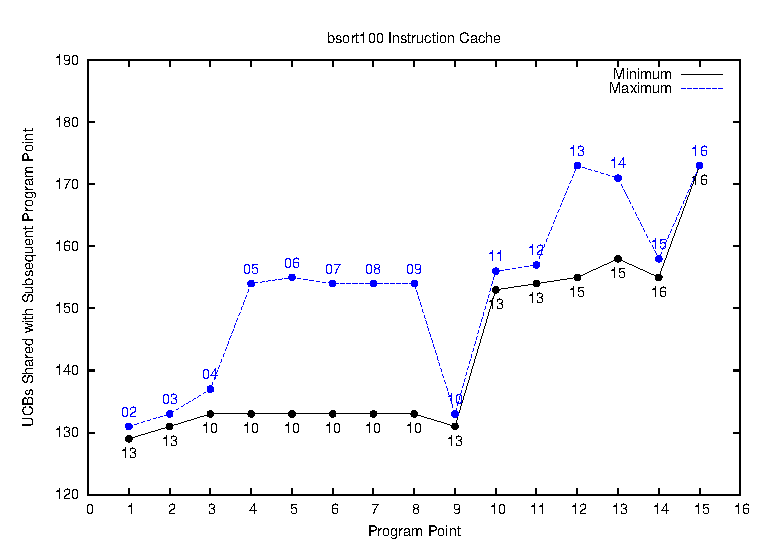
\includegraphics[width=\linewidth]{eps/bsort-icache.eps}
\end{center}

\begin{center}
  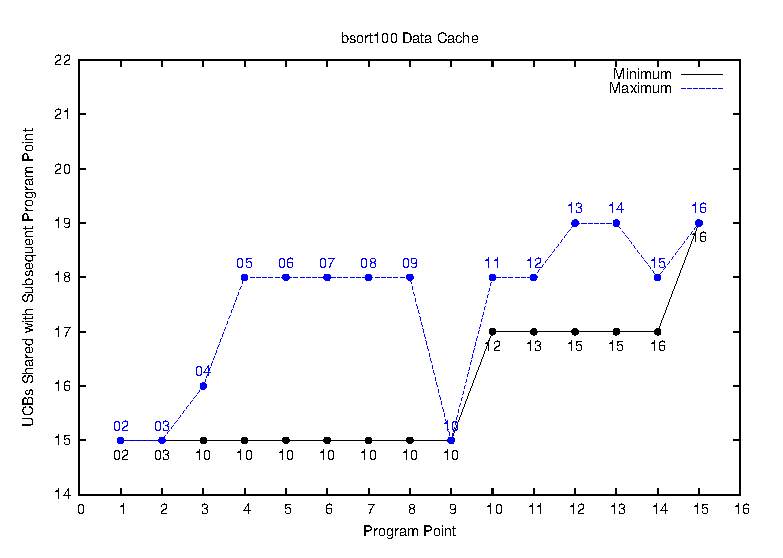
\includegraphics[width=\linewidth]{eps/bsort-dcache.eps}
\end{center}

\begin{center}
  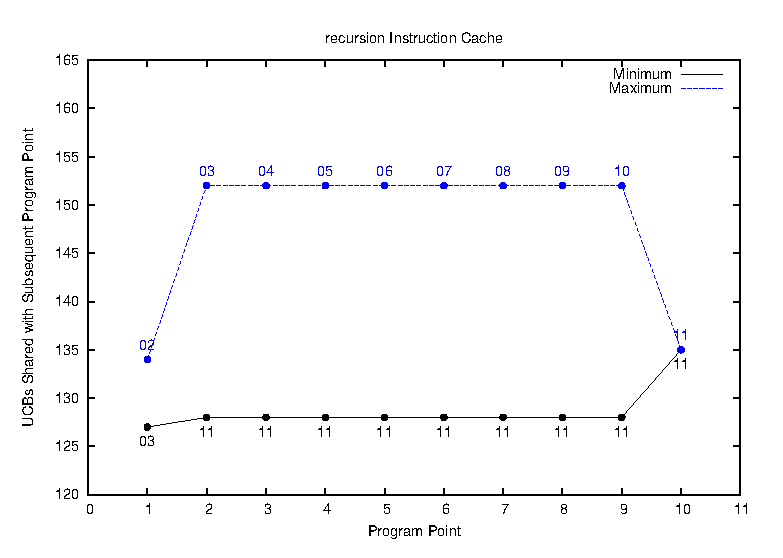
\includegraphics[width=\linewidth]{eps/recursion-icache.eps}
\end{center}

\begin{center}
  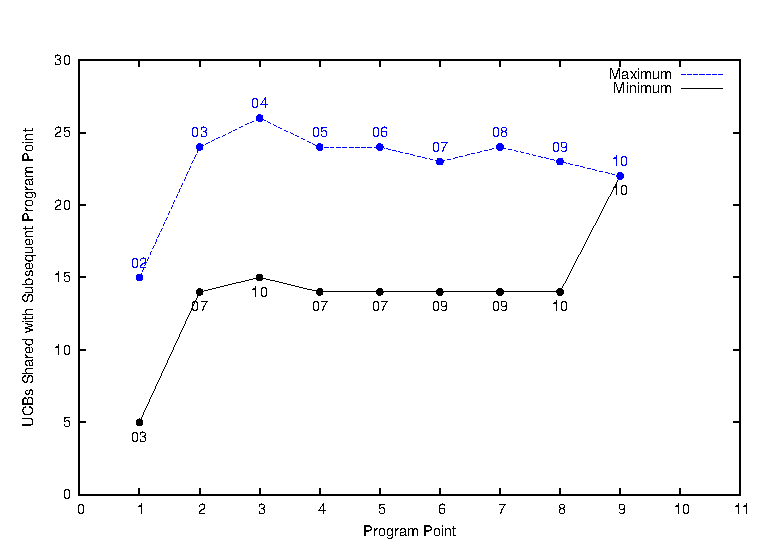
\includegraphics[width=\linewidth]{eps/recursion-dcache.eps}
\end{center}

%% An alternative for a wider graph
%% 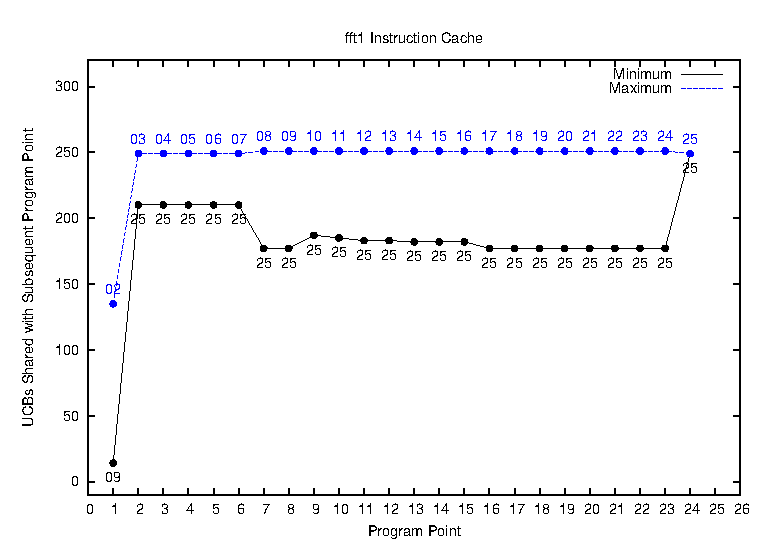
\includegraphics[width=\linewidth]{eps/fft1-icache.eps}

\begin{center}
  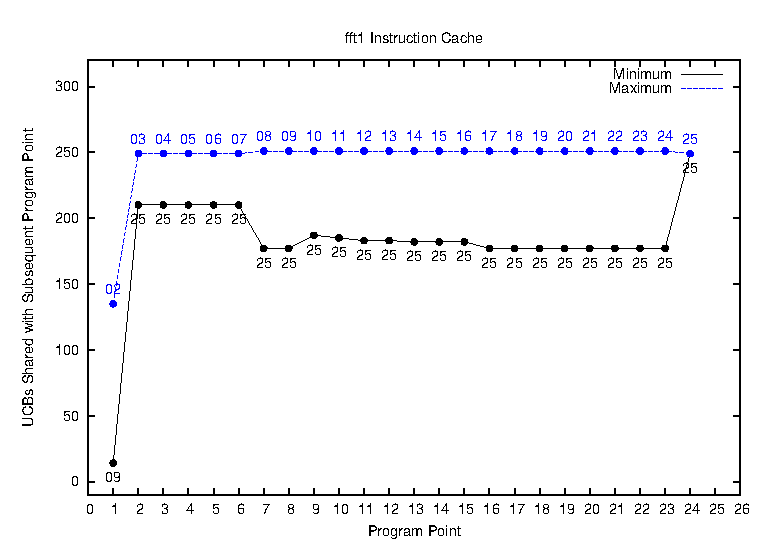
\includegraphics[width=\linewidth]{eps/fft1-icache.eps}
\end{center}

\begin{center}
  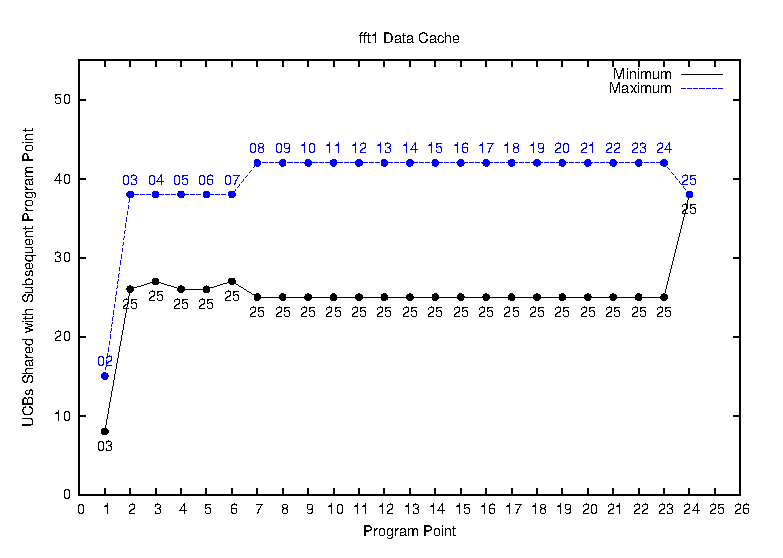
\includegraphics[width=\linewidth]{eps/fft1-dcache.eps}
\end{center}

For the bsort task, the proposed approach provides a benefit for the
instruction and data caches of 2 and 0 UCBs. For the fft1 task, the
instruction and data cache benefit is 121 and 7 UCBs. For the
recursion task, the benefit is 7 and 10 UCBs.

\section{References}

\begin{enumerate}
\item MRTC Benchmarks \\
http://www.mrtc.mdh.se/projects/wcet/benchmarks.html

\item Gaisler Compiler  \\
http://gaisler.com/index.php/downloads/compilers

\item Gaisler GRSIM \\
http://gaisler.com/index.php/products/simulators/grsim

\item AbsInt a\textsuperscript{3} WCET Tool \\
http://www.absint.com/a3/index.htm
\end{enumerate}




\subsection {Taskset Schedulability Evaluation}\label{sec:taskset schedulability}
The schedulability performance metrics we intend to compare various
preemption models with are: 1) the percentage of schedulable task sets
as a function of the task set utilization, 2) the percentage of
schedulable task sets as a function of the number of tasks, 3) the
percentage of schedulable task sets as a function of the maximum CRPD,
and 4) the percentage of schedulable task sets as a function of the
variability of the CRPD variance \begin{math}\sigma_{CRPD}\end{math}.
The following preemption models will be studied namely: 1) fully
non-preemptive, 2) fully preemptive, 3) limited preemption naive
approach, 4) limited preemption point placement with fixed CRPD
preemption cost, 5) limited preemption point placement with variable
CRPD preemption cost, and 6) optimal preemption point placement with
enhanced CRPD preemption cost. 

Our approach for generating the synthetic task sets involves a number
of steps which is summarized as follows.  The number of basic blocks
generated each task is in the
interval \begin{math}[N_{i}(min),N_{i}(max)]\end{math} using a random
uniform distribution.  Each basic block non-preemptive WCET is
generated using a Gaussian distribution with
mean \begin{math}\mu_{WCET}\end{math} and
variance \begin{math}\sigma_{WCET}\end{math}.  The  utilization of
each task has been generated using the approach proposed in [TBD12].
The task periods \begin{math}T_{i}\end{math} were then computed
dividing the non-preemptive WCET \begin{math}C_{i}^{NP}\end{math} by
the utilization \begin{math}U_{i}\end{math} of each task.  Preemption
costs were randomly generated using the following function (TBD), to
achieve a realistic distribution similar to the one derived
empirically).  The enhanced CRPD is generated to be a percentage of
the WCET in the interval [0, 0.50] with a random uniform
distribution. Cache related preemption delay (CRPD) values are
generated for each pair of potential preemption points.  The variable
CRPD preemption cost model uses the CRPD cost from the each preemption
point to the end of the task. The fixed CRPD preemption cost model
uses the maximum CRPD cost of all variable CRPD preemption cost
values.  
